\documentclass{UoYCSproject}
\usepackage{outlines}
\usepackage{tikz}
\usepackage{booktabs,multirow}
\usepackage{graphicx}
\usepackage{subcaption}
\usepackage{amsmath,amssymb}
\usepackage[ruled,vlined]{algorithm2e}
\usepackage{pdfpages}
\addbibresource{bibl.bib}
\author{Angel Simeonov}
\title{Networks and Dragons: A data-driven approach to procedural dungeon generation}
\date{\today}
\supervisor{Dr. Rob Alexander}
\BEng

\dedication{<insert dedication>}

\acknowledgements{
  <insert acknowledgements>
}

% More definitions & declarations in example.ldf

\begin{document}
\pagenumbering{roman}
\maketitle
\listoffigures
\listoftables
%\renewcommand*{\lstlistlistingname}{List of Listings}
%\lstlistoflistings

\begin{summary}
>At most two (2) pages, aimed a non-specialist, knowledgeable authorial peer.
The summary must:
--state the aim of the reported work,
--motivate the work,
--state methods used,
--state results found, and
--highlight any legal, social, ethical, professional, and commercial issues as appropriate to the topic of study (if none, then this should be explicitly stated).
\end{summary}

\chapter{Introduction}
\label{cha:Introduction}

\section{Role-playing games}

\paragraph{}
Role-playing game (RPG) is a broad term encompassing a multitude of different games with often distinct mechanics and media of interaction. The common factor between all RPGs is that the player(s) portray a fictional character in a fictional world (or a subset of one). The interaction of the players with this world is governed by rules, defined by the media. To better understand the structure of RPGs, we can view it in terms of two sets: 
\begin{outline}[enumerate]
  \1 Rules defining how we play the game which describe the allowed actions for the player at any given moment in the game.
  \1 Narrative elements which provide the \textit{purpose} of the players to interact with the fictional world. 
\end{outline}
The first set can be viewed as "How I interact with the environment" (functional) and the second as "What is the meaning of the environment" (narrative).

\paragraph{}
Computer RPGs like the Action RPG (ARPG) Legend of Zelda \parencite{game:LoZ}, Diablo \parencite{game:Diablo}, Fallout \parencite{game:Fallout} and many alike have both sets of rules defined by the game designers. A functional rule in an RPG like Skyrim \parencite{game:Skyrim} is that you can attack with the left mouse button and a story element is that you are a hero with a quest. This quest is defined by the writers and designers of the game and as such exploring the narrative in a digital RPG can be comparable to an interactive reading of a fiction book. Good computer RPGs often have the ability to relax the narrative \parencite{TychsenGM}, allowing for players to have more freedom in the exploration of the world and as such create the sensation that they have impact on this pre-programmed fictional environment.

\paragraph{}
The ability for a player to influence the narrative is one of the defining features of tabletop RPGs (TRPG a.k.a pen-and-paper PnP) like Dungeons and Dragons \parencite{DnD}. In them, the functional rules are usually defined by a rulebook (like the Player’s Handbook) and players verbally describe their interactions with the environment. The narrative is an ever evolving amalgam between the input of players and the Dungeon Master (DM). The DM’s task is to create a narrative outline and guide the player interaction. Because of the verbal nature of the game, the narrative does not suffer the limitations of its digital counterparts. But because there are no hard constraints to how the narrative is told, the DM has the non-trivial task of introducing consistency and outlining a structure for the story that would result in a compelling and ideally immersive experience for the players. This is often achieved by focusing the adventure’s act on a particular and detailed location. These locations are often referred to as Dungeons and in practice can be anything from the villain's mansion or a beast’s cave to a city under siege. A good dungeon design is crucial for creating a compelling narrative. The creative task of making the Dungeon is a laborious process. To facilitate that, academics and various gaming communities have been exploring different ways of automating Dungeon creation. We will refer to this process as Procedural Dungeon Generation (PDG). Arguably the greatest problem posed by automating PDG is answering the question of “What is a compelling Dungeon?”. In the next section we will review different PDG methods and their associated limitations in an attempt to answer this question.

\section{State of the Art Generative methods}
% \begin{outline}
%   \1 Review various different algorithms for PDG and discuss their take on solving the "is this dungeon interesting?" problem.
%     \2 Non-digital: [[the Advanced DnD DM design kit book 3: Adventure Cookbook]]. Using dice tables to create different elements of the dungeon. Laborious process which requires the DM to remove any inconsistencies. Does not provide an actual Dungeon structure.
%     \2 Cellular automata: donjon \parencite{donjonPDG}. Issues associated with completely random topology and random content generation. Evaluated only on if the level is solvable (no evaluation of semantic content).
%     \2 Constraint Propagators and their related issues when formalising narrative as constraints.
%     \2 BPTs + semantic additions[[citation needed Thrall and Brown]]. Difficulty proving the 'goodness' of the generator. Discuss difficulties with an objective HCI evaluation for PnP (i.e. difficult to get a decent sample size, because playing a game is time consuming).
%     \2 Formal language approach. Grammars \parencite{DormansMS,Deery,Cadogan} as a natural way of describing narrative structures.
%     \2 Data-driven approaches. \parencite{SummervilleLearningOfZelda,SummervillePCGML,SummervilleSamplingHyrule} Relate the notion of learning from human-made dungeons as a way to create good structure + narrative. Note the lack of data. Expand more in the Mission and Space --> Aim sections
% \end{outline}
\subsection{Non-digital Generators}
\label{subsec:NDGenerators}
\paragraph{}
The designers of the classic PnP modules acknowledge the issue of Dungeon creation and often incorporate \textit{Loot} or \textit{Encounter} tables in the rule-books. The tables are a reference over a set of treasures or monsters respectively, which can be chosen by rolling the specified die (example in appendix B fig \ref{fig:loot_table}). As noted before, a PnP RPG can evolve rapidly outside the planned narrative structure prepared by the DM and a simple way to quickly generate new adaptive story elements via loot tables can be useful. Some early modules even provided a step-by-step guide for creating a full campaign from the plot, villains' obsessions and story setting to the various encounters and and treasures \parencite{ADnD} entirely based on randomised content tables. An issue arises with using loot tables when a randomly selected element from one table is contradicted by an item selected from another. It is up to the DM to resolve such disparities. Although this process provides some degree of creative assistance, it does little to facilitate the laborious nature of creating an end-to-end compelling narrative. Furthermore, as these methods are occupied with providing inspiration for global narrative elements, they pay no attention to providing guidance of what would mean a "good" Dungeon.

\subsection{Digital Generators}
\label{subsec:DigGen}
\paragraph{}
It is important to note that PnP RPGs and the various genres of computer RPGs share the same narrative goal despite differing in mechanisms of interaction \parencite{Tychsen2006}. Therefore we will not limit ourselves to looking only at existing tabletop solutions.
Unlike the original non-digital generators, computerised ones rarely allow for human input during the generation process. A generative algorithm would provide a DM with an interface that takes a set of input parameters and produces a template of a game. The degree of complexity of this template is dependent on the complexity of the algorithm itself. Because they aim to exclude the human designer from the process, the digital generators tend to focus on creating elaborate Dungeon structures and either provide basic narrative content or omit it entirely.

\subsubsection{Cellular Automata}
Cellular automata (CA) utilises a procedural generation mechanism in which a $N \times M$ grid space is mutated incrementally by a set of agents. The implementation of these mutation operators define if the CA will simulate erosion \parencite{donjonCA} or man-made structures such as rooms with corridors. An example that can accommodate both can be seen in the donjon dungeon generator \parencite{donjonPDG}. Its simplicity and degrees of customisations of layout and style has made donjon a popular generator choice. At time of writing, it has more than 2500 generated dungeons in the last 12 hours and 100 donations in the last 3 months. Despite its popularity, donjon (as well as other CA PDGs) implores purely random generation techniques which are only evaluated based on the reachability (i.e. is there a path from the start to each room). Furthermore, although we have control over the input parameters for the topological randomness, the narrative elements (the contents, rather than the structure) of the dungeon are entirely arbitrary and often contradictory \parencite{Thrall,Brown}. In terms of the aforementioned reachability, donjon does not take in account the randomly allocated locked doors as the key allocation is left at the DM's discretion. That ultimately limits the usefulness of the tool as a narrative generator. %All information generated about the monsters, treasures and other quest elements are discarded by the DM \textbf{[[citation needed on how people use dungeon generators]]}

\subsubsection{Constraint Propagators}
Constraint Satisfaction Problems (CSPs) define a discrete set of variables with corresponding constraints that restrict the possible variable instantiations \parencite{kumar1992CPalgorithms}. PDG has been described as a CSP on occasions where the variables and constraints define the layout \textbf{[[cn]]}, contents \parencite{HorswillCSPMission} or both layout and content \parencite{GreenCSPboth} of a dungeon. Constraint Propagation (CP) is a particular method proven useful for solving CSP in the context of PDG. The algorithm randomly selects a set of possible values for a particular variable and \textit{propagates} the result to the rest of the variables, adjusting their possible values accordingly. If the selected value narrows another variable's possible values to the empty set, we infer that this instantiation is suboptimal and we backpropagate to the last viable solution and retry. Furthermore it can be generalised that a level is solvable if an instantiation exists such that no variables are reduced to the empty set. Utilising this formalisation of the \textit{solvability} of a level we can populate a dungeon with varying degrees of complexity from ensuring that keys are always spawned before the door that they unlock to adjusting difficulty by measuring survivability metrics between rooms. Even thought CPs have solved some problems of the purely random generators, formulating a numerical constraint for a narrative element can be difficult. The complication is both in the translation of a story element to a numerical representation and in the computational expense that comes with computing large amounts of permutations.

\subsubsection{Context aware Binary Space Partitioning}
\label{subsub:BSP}
Other methods proposed by Thrall \parencite{Thrall} and Brown \parencite{Brown} use a Binary Partitioning Tree \parencite{BSP} to create the layout of the dungeon. The simplicity in randomly dividing a 2D space until we have the desired number of rooms allows them to focus on the narrative content of the dungeon. Apart of just specifying layout parameters as is the case for the donjon generator, they attempt to be contextually aware of the game's narrative. Examples are tailoring loot for specific players or noting that noise in a certain room will provoke monsters from nearby ones. Although this is a step towards narrative automation, these elements are very basic. This leads to the necessity of the DM to refine the result of the generation and occasionally ignore it completely. An example of a case where the narrative guide makes no sense would be a room labelled as provoking, yet no nearby rooms host monsters. Thrall and Brown's PDG can be viewed as a digital version of the classic PnP generators we discussed in section \ref{subsec:DigGen} and as such incur the same issues. Furthermore, Thrall and Brown have shown that evaluating the \textit{goodness} of a PDG method is a complicated task. A purely HCI evaluation of the qualities of a dungeon is understandable, but a single game of PnP RPGs takes on average 3-4 hours \parencite{gameSessionLengthPoll} making it very difficult to get a representative sample size in a short period of time. This implores considering the trade-off between environmental validity and practicality when designing a user study for evaluating PDG methods for tabletop RPGs.

\subsubsection{Formal Languages}
\label{subsub:FL}
A natural way to encode contextual meaning and structure has made formal languages for PDG and object of interest to several researchers \parencite{DormansMS,Cadogan,Deery}. Namely generative grammars enable a designer to specify a set of production rules with arbitrary complexity that dictate the sequence in the PDG process for both layout and contents of a dungeon. A critical consideration when using grammars is the issue of what vocabulary of dungeons is a particular grammar set going to produce. Cadogan \parencite{Cadogan} created a baseline grammar based on some logical heuristics, but it does not differ in output from a parameterised random PDG. Deery used a more analytical approach to grammar rule selection by manually analysing submissions to the One Page Dungeon Contest \textit{OPDC} \parencite{OPDC} and noting any common patterns. His noble aim was to transcribe common patterns as grammar production rules in an attempt to make the generator produce dungeons with elements that exist in human-made ones. Although a very interesting proposition, it required several important restrictions to be viable in practice. Namely he focused only on the narrative content i.e. what the players have to do to finish the dungeon and disregarded the level topology entirely. The generator proceeds to map the narrative content to a usable layout in a 1:1 ratio, resulting in a single task per room. It is trivial to see that the originals in OPDC do not impose such a restriction. One room can have multiple narrative elements (e.g. the key to unlocking the door is on the bandit’s waist, Key + Encounter). Furthermore, Deery’s approach was to manually look at 10 competition winners and heuristically extract the grammar rules, which he highlights that they do not capture all possible patterns.

% Deery \parencite{Deery} made the first steps by manually analysing submissions to the One Page Dungeon Contest \textit{OPDC} \parencite{OPDC} to extract a graph grammar for Mission generation. The Mission graph was then mapped to a physical Space in a 1:1 ratio. The result was that each room was limited to a single Mission element. It is trivial to see that the originals in OPDC do not impose such a restriction. One room can have multiple Mission elements (e.g. the key to unlocking the door is on the bandit’s waist, Key + Encounter). Furthermore, Deery’s approach was to manually look at 10 competition winners and heuristically extract the grammar rules, which he highlights that they do not capture all possible patterns. An automated approach to learning would potentially solve that issue.

\subsubsection{Data-driven approaches}
\label{subsub:DataDriven}
 Arguably one of the most pleasant gameplay experiences in tabletop RPGs spring from exploring intricately structured dungeons and their mysteries. Their compelling features are due to the fact that they are made by a human designer that understands the needs of the players. Researchers have acknowledged that the structure of human-made dungeons should be studied to better answer the question of "What makes a compelling dungeon". Summerville \parencite{SummervilleLearningOfZelda} has shown that extracting features for layout and narrative from the Legend of Zelda games can be automated by training a machine learning ML model on data from the existing, man-made dungeon levels. ML for PDG not only promotes informed content generation, but it can be used as an exploratory mixed-initiative/analysis tool for formalising dungeon structures \parencite{SummervillePCGML}. The other approaches we have discussed have seen applications for both digital and tabletop RPGs, but data-driven PDG is largely an unexplored area. They are especially rare for tabletop RPGs so much that we do not know of publications on ML for PnP RPGS. Presumably this is due to PnP RPGs being virtually unbounded by any functional constraints which makes the task of finding a consistent dataset very difficult.

\chapter{Motivation and Aims}

\section{Mission and Space}

\paragraph{}
An attentive reader would have noted that distinguishing between the level layout and contents is a common occurrence in popular PDG algorithms. This discrimination was formalised by Dormans \parencite{DormansMS} in his definitions of \textit{Mission} and \textit{Space}.
The \textit{Space} of a dungeon represents its topological structure and can be encoded as an undirected cyclic graph where each vertex is a room and each edge is a door or corridor. The \textit{Mission} is the set of narrative tasks the player must accomplish in order for him to complete the dungeon. It can be encoded as a directed graph where each vertex is the objective and the edge directions show the required sequence of completion. How players interact with the level is governed entirely by the overlap of Mission and Space. As noted by Dormans, a \textit{Mission} mapped on different layouts will result in drastically different exploration patterns. By understanding the necessities of the two separate entities we can model player experience better. Due to this separation we have seen advancements in generating adaptable to the player game environments \parencite{DormansAE} and even reverse engineering the creation of \textit{Missions} and \textit{Spaces} by learning structure from data as discussed in \ref{subsub:DataDriven}.

\section{Aim}
\label{sec:Aim}
%\begin{outline}
%  \1 The only \textit{"dungeon generator"} that has been empirically proven to have the ability of creating a truly compelling narrative is the human designer
%  \1 Discuss attempts at the data-driven approaches from \textbf{Generation Methods} in detail
%    \2 Deery's data inspired approach, but not data-driven
%    \2 Summerville's Learning of Zelda
%\end{outline}

\paragraph{}
The dungeon’s topology (Space) and contents (Mission) are correlated and embody the narrative of the game. As we have seen, dungeon generators usually implore bottom up approaches in which they apply rules for topology and then introduce dungeon content in an attempt to provide the structure for a captivating narrative. The various algorithmic methods have clear strengths and shortcomings in achieving the complex goal of creating an interesting story. From these observations it can be argued that that the ultimate \textit{dungeon generator} is the human designer. Dungeons and therefore narratives produced by humans are the most compelling out of all created dungeons. If we implore a top-down approach of recreating good man-made dungeons, we could potentially achieve higher levels of narrative automation. As highlighted by Deery's approach discussed in section \ref{subsub:FL} extracting meaningful information from human-made dungeons and transcribing it in a way that a PDG tool can use it is a very powerful concept. The issues with his approach can be addressed by an automated approach to learning the patterns. Programmatically learning a level from data has been an object of interest for computer based RPGs as seen in section \ref{subsub:DataDriven}, but has not been applied to PnP RPGs, presumably because of the lack of a consistent dataset.

\paragraph{}
In this paper we investigate if applying a data-driven approach to learning the Space of the dungeon can produce a layout that is undistinguishable from human-made dungeon topologies. Choosing Space exclusively is due to the fact that it is more universally consistent than Missions which will aid us in managing the scope in this already time constrained environment. Inspired by work on digital RPGs, we discuss how we can use inference (Bayesian) networks to learn Space features from data. A review of the availability of data is conducted and complemented by assessing how meaningful features can be extracted. Subsequently we compare different network structures and learning algorithms and internally assess which model has the greatest statistical predictive capabilities using two scoring rules. We examine different methods that we can use for generating a dungeon topology from the best performant inference model. We conclude with a user study on preference to externally validate how well the generator has approximated human-made dungeon topologies.

\chapter{Bayesian Inference Networks for PDG}
\label{ch:BNETS}
\paragraph{What are Bayesian networks?}
Bayesian Networks \textit{BNs} \parencite{pearl1985bayesian} (also referred to as Inference Networks, Belief Networks or Directed Acyclic Graph \textit{DAG} Models) are a graphical probabilistic model in which vertices are random variables \textit{RVs} whose edges indicate causal beliefs. BNs assert that our domain is defined in terms of a joint probability distribution \textit{PD} \(P(X_1, \ldots , X_n)\) over a finite set of RVs \(X\), each of which has a set of potential values it can take \(X_i(\Omega) = \{x_1, \ldots, x_j\}\) with an associated PD. The network structure shows how the full join distribution factorises given the causal dependencies. This property gives us a way to encode our prior domain knowledge about the relationships between our RVs.
Once we have encoded the RV interaction, using a BN as an inference tool is a matter of querying with a conditional set of RVs and noting how the conditional probability tables \textit{CPTs} change given our new knowledge. In practice, conditioning is done by \textit{observing} (i.e. instantiating) an RV to a particular value. Extracting information from our newly formed conditional distributions is done by sampling. Sampling involves simulating our network with respect to the observations in order to obtain point estimates. A detailed discussion of the sampling methodology will be provided in section \ref{sec:implementation}.

To contextualise the inference process for PnP RPGs, we can look into Summerville's work on the ARPG Legend of Zelda dungeons \parencite{SummervilleLearningOfZelda}. After annotating the dungeon maps with elements of both Mission and Space (total number of rooms, treasures, monsters, the length of the optimal path from entrance to goal, i.e. the \textit{critical path CP} and others), he extracts features for the BN by parsing them as RVs. Conditioning on total number of rooms by stating \(P(NumRooms = n) = 1\) results in a change of the PD for the possible CP values. An example logical outcome would be that the CPs that are greater than the total number of rooms would become impossible \(P(CriticalPathLength > n \mid NumRooms = n) \rightarrow 0 \). Then by sampling the network a point estimate for critical path length given that number of rooms in the dungeon is extracted. This \textit{observe-then-infer} process can be done with any permutation of our RVs.

\paragraph{Why use Bayesian networks?}
% causal structures gives us a natural interpretation of complex non-linear problems, compared to other methods (think NNs and their inability to be interpreted)
% they are fast once trained. Updating belief is a simple arithmetic operation on the different CPT
% gives us precise control over the parameters. Deery had an approximation of how big a dungeon should be because he would just repeat the rules X number of times. We can precisely fix every parameter that we have and even do permutations. This gives new degrees of freedom for the user to select the desired properties of his dungeon without compromising on automation.
The reasoning behind choosing BNs is that the probabilistic causal structures have been shown to perform well in capturing structural properties of dungeons from data for PDG tasks in digital RPGs \parencite{SummervilleLearningOfZelda,SummervilleSamplingHyrule}. Furthermore they give us a natural description about the dependencies in our model, which can be used as a supplemental analysis tool for investigating human-made dungeons. As a PDG tool itself, the \textit{observe-then-infer} pattern gives the user precise control over the desired properties of his dungeon without loss of automation. If a user observes a dungeon with 5 rooms and critical path of length of 3, they will be guaranteed in the final product. This solves the problem previous graph grammar data-driven approaches encountered, whereby the dungeon size input was used as an approximation for the actual number of rooms in the dungeon \parencite{Deery}.

The downside of BNs is that their generalisation capabilities are highly dependent on the availability of data. If conditioning on an \textit{undefined} set (e.g. there was never a data entry that showed a 5 room dungeon with CP of 3), the inference will fail. Fortunately there are ways to work around this problem which we will discuss in section \ref{subsec:feature_extraction}.

A proposed way to solve this issue is by creating artificial data entries for the undefined cases. We will use linear interpolation due to its simplicity and the fact it has been shown to produce good results in general \parencite{Ibargengoytia2013OnTE} and exceptional results on small datasets \parencite{yu2004advances}. This can potentially solve the problems of undefined dungeons within the range of sizes of our dataset, but it cannot extrapolate to infer arbitrarily large dungeons. We would like to argue that this generalisation restriction is not a limitation of our algorithm, but of the data. Different dungeons exhibit different properties and it is not feasible to consider learning all possible existing dungeon configurations from a single dataset. This limitation is reflected in the dataset selection criteria in the next section.

\chapter{Methods and Implementation}

%ToDo: Finish summarising key assumptions, and models
\paragraph{}
In this section we explore various issues with formalising the conversion of human-made dungeons to probability distributions for use with our Bayesian networks. The key assumption we propagate throughout this section is about the parallels between digital and tabletop RPGs we made in section \ref{subsec:DigGen}. This assumption allows us to base feature selection and model architecture based on previous work done by the ML community. We discuss Bayesian network architectures in three different levels of complexity and two different parameter learning algorithms.

\section{Data acquisition}

\paragraph{Note on notation}
\begin{outline}
  \1 \textit{Features} or \textit{RVs} are denoted by capital letters \(X\) where a boldface \(\boldsymbol{X}\) is a shorthand for a set of RVs \(\{X_1, \ldots, X_n\}\)
  \1 \textit{Parameters} refer to the Bayesian network parameters, i.e. the conditional probability tables CPTs defined by the different RV dependencies \(P(Y_1, \ldots, Y_n \mid X_1, \ldots , X_n)\)
  \1 Joint probability distributions \(P(X_1, \ldots , X_n)\)
  \1 Calligraphic \(\mathcal{N}\) is a shorthand for the parameters for a given network
  \1 Calligraphic \(\mathcal{D}\) is a wrapper for all the RVs (i.e. our data)
\end{outline}

\subsection{Data selection} % what dataset should we choose:: OPDC winners for the last five years
% What problems can we encounter? Sparsity of data. Very different dungeons, some are unusable (say unusable criteria)

\paragraph{}
Unsurprisingly the first priority of a data-driven method is the acquisition of a suitable dataset. The criteria we have chosen for our data is the following:
\begin{outline}[enumerate]
  \1 Data must be consistent. Dungeons have to be logically comparable.
  \1 Data must be available under a research or similar open-source license.
\end{outline}
The \textit{OPDC} supplies a dataset that satisfies our requirements. All dungeons are in the same category of a one-session long dungeon and each dungeon is issued under the Creative Commons CC license. Furthermore due to the fact that it is a competition, we have an exemplar answer of our main question "What makes a compelling dungeon?" in the form of the competition winners. We apply the first filter and review only entries by competition winners. Due to the creative freedom the human designers have, it is na\"{i}ve to assume that the dungeon Space is necessarily a dominant factor in all dungeons. In order to narrow down to dungeons that do have a consistent representation of Space as an important asset, we apply a second filter by omitting dungeons that have:
\begin{outline}[enumerate]
  \1 no map (no Space)
  \1 exclusively linear topologies
  \1 non-standard Space traversal (the map topology is ignored due to a functional mechanism e.g. time-travel, game of political control, king of the hill, etc.)
  \1 inconsistent map (our Space features change as the game progresses e.g. intrigue campaigns where the objective constantly changes locations)
  \1 no goal defined by the designer (introduces the same problem as 4.)
\end{outline}

\subsection{Extracting Features}
\label{subsec:feature_extraction}
\paragraph{}
We will base our feature selection on the work done by Summerville we discussed in section \ref{subsub:DataDriven}. He showed that his Extreme Sparse model (seen in fig \ref{fig:SESM}) not only has the greatest predictive capabilities, but is also the least complex model, having only 10 features. As a corollary from our assertion that digital RPGs do not differ from tabletop RPGs in terms of dungeon design philosophy, we can assume that the predictive capabilities of the Extreme Sparse model will be similar if applied in PnP context. As noted in section \ref{sec:Aim}, we will focus on Space related variables, disregarding Mission due to its inconsistency in PnP dungeons. This crucial reduction can be detrimental to the predictive capabilities of the model, but it is a necessary step to introduce the prerequisite consistency for the ML task as discussed in the previous paragraph. Incorporating Mission features in our model would mean further reduction of the already small dataset. The resultant selection uses the top five explanatory Space RVs split in two categories: 
\begin{outline}[enumerate]
  \1 Dungeon (Global): total number of rooms \(R\) and how many rooms form the shortest path between the entrance and the goal (the \textit{critical path CP})\(L\)
  \1 Room (Local): depth \(D\) (how far away the room is from the entrance), critical path distance \(S\) (how far away is the room from a critical path room, 0 indicates it is on the CP) , total number of neighbours \(N\)
\end{outline}
The chance of a particular RV taking some value is dictated by an unknown PD. As our RVs are related, it is logical to describe our dungeon as the interaction of the different RV PDs. That means that we can describe this unknown PD for a full dungeon by composing the global and local parameters in a joint PD. More formally, each global and local set of features is defined by the joint PDs respectively \(P(R, L)\) and \(P(S, D, N)\), where each variable is discrete. A full dungeon is therefore characterised by 

\begin{equation}
  \label{eq:full_joint_PD}
  P(R,L,S,D,N) = P(R, L) \prod_{r}^{\mid R \mid} P(S_r, D_r, N_r)
\end{equation}
where \(|R|\) is the total number of rooms defined by the instantiation of \(R\). This reads that the probability of having a particular dungeon is dictated by the interaction of the of the size and CP length with each individual room. Each of terms on the LHS is unknown and we need to \textit{learn} them from the OPDC data. To do so, we extract these five features by transforming the artistic and graphically rich textual representations of the OPDC dungeons to a computer readable representation. Unfortunately automating feature extraction is very difficult due to the variant stylistic formatting and the prose like description of the tasks. Because of this, we establish a systematic way of manually annotating the Space of the dungeon as an abstract undirected graph from which we can calculate all the different features (see Appendix A for example \ref{fig:SOTA}).

\paragraph{}
The dungeon sizes in our dataset range from two to 27, but due to our restrictions combined with chance, dungeons of some sizes were never recorded. Namely dungeons with sizes \(\{4,23\}\). We could conclude that lack of dungeons from those sizes means they are highly improbable to the point where we should not be concerned with their existence. This is what we do with dungeons that are outside of the range of sizes for one-page adventures. But in terms of utility of our tool we would like to be able generate any dungeon within that range. This issue of undefined data is the main drawback of inference network as outlined in chapter \ref{ch:BNETS}. Our proposed solution is to linearly interpolate \textit{LI} dungeons that are close to the missing ones in order for us to get estimates for the global RVs. We have chosen LI due to its simplicity and the fact it has been shown to produce good results in general \parencite{Ibargengoytia2013OnTE} and exceptional results on small datasets \parencite{yu2004advances}. Room (local) RVs could potentially also be linearly interpolated by using all the rooms from the neighbouring dungeons but this poses several questions about what does it \textit{mean} to interpolate 4 rooms and 6 rooms. A better and more intuitive way to handle them is by leveraging the properties of the BNets. We can represent the rooms for the interpolated dungeons as unknown values to be inferred from the known data. We are treating the data itself as a parameter to be estimated from our other observations. This is a convenient way that inference networks treat missing values or sometimes even missing variables \parencite[p45]{neticaCman}. However this representation of the unknown will impose a restriction on what CPT learning algorithms we can use. We discuss them in section \ref{subsec:param_learning}.

\paragraph{}
The final dataset is saved in a CSV format \texttt{DR\_data.csv} and consists of 92 dungeon + 1193 room entries and 10 linearly interpolated dungeon entries with 189 unknown rooms. Common statistics of the dataset can be found in appendix \ref{cha:aA}.

\section{Model selection} % we have to choose a model structure denoting assumptions about dependencies then compute the CPTs
\label{sec:model_selection}

\paragraph{What we need to do to use Bayesian Networks?}
We need to define two key attributes of the BN:
\begin{outline}[enumerate]
  \1 The causal network's topology
  \1 The network parameters
\end{outline}
In this paper we will empirically compare different models in search of the one with highest statistical predictive capabilities. We will evaluate three structures with two CPT learning algorithms against a uniform distribution (control) for a total of 7 models. The structures are the previously discussed Extreme Sparse model (modified for Space only), an automatically learned structure using the Tree Augmented Na\"{i}ve Bayes and a fully connected model. The three architectures are chosen as such because each one differs in complexity and in assumptions. The comparison is an exploratory experiment aiming to see which pair of complexity and assumptions fits the OPDC data best. In regards to parameter learning, the CPT learning algorithms will be Expectation Maximisation \textit{EM} and Gradient Descent \textit{GD} due to their ability of handling missing data. Implementation of all BN related algorithms is done in the Netica Bayesian Network development software \parencite{netica}.

\subsection{Bayesian Network topology}
\subsubsection{Summerville's Extreme Sparse Model \textit{SESM}}
In section \ref{subsec:feature_extraction} we discussed the usefulness of the high accuracy SESM for small datasets (Summerville's original model was trained on 38 dungeons with 1031 rooms). The first BN topology we will therefore consider is a flattened to Space features only SESM. The flattening is done by reconstructing the SESM in Netica and applying the \texttt{AbsorbNodes\_bn} \parencite[62-63]{neticaCman}. The function removes the unused Mission RVs by effectively treating them as constants and propagating any implied dependencies from the other nodes. In this way we remove the unused RVs and maintain the joint distribution dependencies between our Space features. The transformation can be seen in figure \ref{fig:ExpertBNet}. The resulting model describes the following factorisation over our RVs:
\begin{equation}
  \label{eq:SESM}
  P(R,L,S,D,N) = P(R)P(S)P(L \mid R)P(D \mid R, L)P(N \mid D, S)
\end{equation}

\begin{figure}[htb]
  \centering
  \begin{subfigure}[b]{0.55\textwidth}
    \centering
    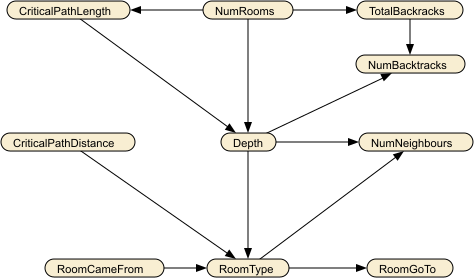
\includegraphics[width=\textwidth]{SESM_full.png}
    \caption{Summerville's Extreme Sparse Model}
    \label{fig:SESM}
  \end{subfigure}
  \hfill
  \begin{subfigure}[b]{0.35\textwidth}
    \centering
    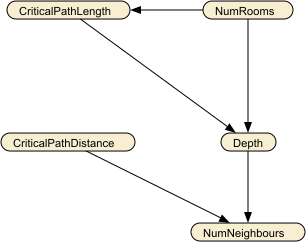
\includegraphics[width=\textwidth]{SESM_space.png}
    \caption{Space only Model}
  \end{subfigure}
  \caption{Expert defined Network topologies}
  \label{fig:ExpertBNet}
\end{figure}

\subsubsection{Tree Augmented Na\"{i}ve Bayes}
% In the above approach we used specialist knowledge (Summerville's experiments) to create the BN structure
% We made two crucial assumptions in that PnP == ARPG && flattening Mission to Space only will still retain the same operational meaning of the dungeon due to it retaining the same conditional dependency assumptions through the BN properties
% But we want to put those assumptions to the test by also learning the graph structure from the data we have.
\paragraph{}
In the above approach we applied specialist knowledge from Summerville's experiments to create the BN structure. For that network to be valid, we made two assumptions: equivalence between PnP and ARPG dungeons and that flattening Mission to Space retains the same operational meaning due to the BN retaining the same conditional dependencies. To contest these somewhat ambitious assumptions, we will also create a BN by ignoring any domain knowledge we have and infer the structure purely based on the data using Tree Augmented Na\"{i}ve Bayes \textit{TAN} \parencite{FriedmanTAN}.
\paragraph{}
Informally the learning procedure can be defined as finding the most likely BN structure that \textit{agrees} with our data. That means we are searching for the network structure that is most likely to have been produced given the data. TAN finds the most likely network structure in two steps:

\begin{outline}[enumerate]
  \1 Start with a universal model (Create a na\"{i}ve Bayes model)
  \1 Find correlated variables in the data and connect them with causal edges
\end{outline}

The universal model TAN chooses is the standard na\"{i}ve Bayes. It asserts that all RVs are conditionally independent given one specific RV (the class RV). We will choose the class to be \(R\) due to its contextual importance. The na\"{i}vity assumption implies that
\begin{equation}
  \label{eq:TAN}
  P(R,\boldsymbol X) = P(R)\prod_{x}^{\boldsymbol X} P(x \mid R)
\end{equation}

where \(\boldsymbol X = \{L, S, D, N\}\). With this very restrictive assertion we have a usable BN structure. The conditional independence given the class variable is useful in practice and has been shown to produce competitive results \parencite{RishEmpiricalBayes}, but the operational meaning of this assumption might cause issues if we use it as is. Namely we are assuming that as long as we know how big the dungeon is, the room variables (depth, critical path distance and neighbours) do not influence one another, which does not make much sense. For precisely this reason, the TAN algorithm analyses our data and creates \textit{augmenting edges}. They are causal links connecting RVs that are found to have correlations. The resultant network has an informed causal structure and is alleviated from the restrictions of the na\"{i}ve assumption. The networks resulting from each of the two steps can be seen in figure \ref{fig:TAN}.

%It should be noted that the we did not discuss the \textit{tree} nature of TAN, because it is related to practical optimisations for learning large graphs with which we are not concerned.

\begin{figure}[htb]
  \centering
  \begin{subfigure}[b]{0.43\textwidth}
    \centering
    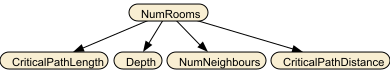
\includegraphics[width=\textwidth]{NBNet.png}
    \caption{Na\"{i}ve Bayes}
  \end{subfigure}
  \hfill
  \begin{subfigure}[b]{0.50\textwidth}
    \centering
    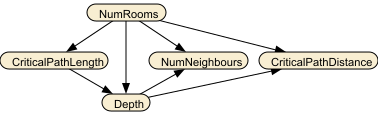
\includegraphics[width=\textwidth]{TANNet.png}
    \caption{TAN}
  \end{subfigure}
  \caption{Learned Network topologies}
  \label{fig:TAN}
\end{figure}


\subsection{Fully Connected}
Due to the fact that we have a small number of nodes, we can afford the computational expense of running a model with no independence assumptions. In effect we're solving the original model \ref{eq:full_joint_PD}, but we will include a heuristic assumption about the direction of the causality in order to maintain the BN requirement of having an acyclic graph. Namely we assert that our global parameters cause our local parameters. The model can be seen in figure \ref{fig:FullyConnected}.

\begin{figure}[htb]
  \centering
    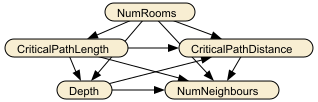
\includegraphics[width=0.7\textwidth]{FullyConnected.png}
    \caption{Fully connected graph with heuristic causal flow}
  \label{fig:FullyConnected}
\end{figure}


\subsection{Parameter Learning}
\label{subsec:param_learning}
When we learn parameters (CPTs for each RV) we are trying to find the most likely PD for each RV that agrees with our data. More formally if \(\mathcal{N}\) is the network's CPTs and \(\mathcal{D}\) is the data then from Bayes's rule we know that \(P(\mathcal{N} \mid \mathcal{D}) = \frac{P(\mathcal{D} \mid \mathcal{N})P(\mathcal{N})}{P(\mathcal{D})}\). We can formulate the parameter learning as an optimisation problem where we find the best values for the posterior \(P(\mathcal{N} \mid \mathcal{D})\) by maximising the likelihood \(P(\mathcal{D} \mid \mathcal{N})\) given our prior \(P(\mathcal{N})\) \parencite[46-48]{neticaCman}. This is in fact the common maximum likelihood estimation MLE \textbf{[[cn for MLE]]}, but because we have missing data, \(P(\mathcal{D})\) is undefined and therefore the MLE is also undefined. To work around this issue and learn the likelihood we review two algorithms Netica has in its toolkit.
 
% \subsubsection{Count \parencite[48-50]{neticaCman}}
% The counting learning states that the probabilities in a single node are defined by how often a particular value has been seen in the data. This notion is defined as the \textit{experience} of that value. The network starts in a state of complete ignorance with uniform probabilities across all RVs. As we iteratively load in the data, the CPT are updated by increasing the probability for a particular value every time it is seen. Specifically, the experience is updated by the previous experience and the degree factor of that data point (i.e how often is it repeated, usually 1) \(e^{\prime} = e + d\). The CPT values are computed as a ratio of the previous and newly observed experience \(P^{\prime}(X=x) = \frac{P(X=x) \times e}{e^{\prime}}\). The counting algorithm is recommended due to its speed and simplicity, but it has a substantial drawback in the fact that it needs the data to be fully defined. Theoretically we should be able to use the counting algorithm as we have no latent (undefined) RVs nor missing data.

\subsubsection{Expectation Maximisation EM}
EM \parencite{EMAlgorithm} is a numerical algorithm that can handle missing data. It assigns random probabilities to our missing values and iteratively alternates between maximising the parameters of the model given the data (Maximisation step) and finding better estimations of the missing data (Expectation step). It converges after a certain set of predefined iterations or when no new updates are happening. 

\subsubsection{Gradient Descent GD}
GD is another algorithm that is able to find parameters for missing data. Netica specifically uses conjugate gradient descent \textbf{[[cn]]} whereby it maximises \(P(\mathcal{N} \mid \mathcal{D})\) by computing the steepest gradient, taking in account the previous one \parencite[p47]{neticaCman}. Both EM and GD risk getting stuck in local optima.

\section{Implementation}
\label{sec:implementation}
\paragraph{}
Obtaining a dungeon is done in three steps, seen in fig \ref{fig:PDGPipeline}. Initially we run the inference process and obtain a set of estimates for all of our features given the size of the dungeon set by the user. We will call the set of estimates our \textit{dungeon configuration}. Subsequently we convert the configuration to an abstract graph by applying a Constraint Propagation algorithm. Finally we convert the abstract graph to a usable dungeon image.

\begin{figure}[htb]
  \centering
    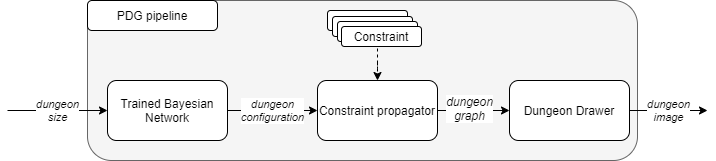
\includegraphics[width=\textwidth]{figures/BPDG_flow.png}
    \caption{Pipeline for the data-driven PDG tool}
  \label{fig:PDGPipeline}
\end{figure}

\subsection{Dungeon configuration}
As we discussed in chapter \ref{ch:BNETS}, generating a dungeon with five rooms is a matter of fixing (\textit{observing}) the \texttt{NumRooms} parameter and inferring the rest. When an RV is observed, Netica updates the CPTs for all dependent RVs with the newly added belief. We can then draw a value from the newly formed distributions. This process of taking a single value from a PD is known as \textit{sampling} the PD. After a value for a previously unknown RV has been sampled, it is added as an observed RV for any subsequent inference. The user can choose virtually any permutation of variables to be fixed or inferred. For consistency of this experiment, we start by observing only the size of the dungeon via \texttt{NumRooms}. Obtaining a dungeon configuration from our model is done in two steps:

\begin{outline}[enumerate]
  \1 Infer the dungeon RVs and validate them (dungeon sampling)
  \1 Infer the room RVs and validate them (room sampling)
\end{outline}


 %from chosen model --> dungeon graph, assumptions about constraints specifics etc
\paragraph{Dungeon Sampling}
 As the size of the dungeon is observed, we only require to sample and validate the CP length. The validation is a sanity check to see if the value for the CP length is not greater than the size. If the validation is successful we continue the inference process. Otherwise we redraw the sample. Formally what we are doing is obtaining a point estimate for the CP length \(L=l\) from the PD \(P(L\mid R = r)\) where \(l \le r\).

\paragraph{Room Sampling}
Once the size and CP length of the dungeon have been observed we can infer the specific room parameters in the same way as before. The validation for room samples is that the depth and number of neighbours cannot exceed the size of the dungeon. If a sample is invalid, we again retry. This is repeated until we have drawn a valid sample for each room in that dungeon. Formally speaking, for each room \(i\) we obtain a point estimate for the room features \((D_i, S_i, N_i) = (d_i, s_i, n_i)\) from the PDs \(\prod_{i}^{r} P(D_i, S_i, N_i \mid R =r, L = l)\) where \(\forall d, \forall n \le r\). The sequence of operations can be seen in Appendix A algorithm \ref{algo:sampling}.
% fix dungeon, sample the rest
% Netica applies the Naive Bayes assumption that given the class variable NumRooms, all rooms are independent. The reason for this assumption is that we avoid the computational complexity of maintaining series of CPTs for each room instantiation. Why is this assumption not bad for us? Potentially because it's empirically shown to not decrease accuracy? https://www.norsys.com/WebHelp/NETICA/X_Bayesian_Learning.htm "Assuming the conditional probabilities to be independent generally results in poor performance when the number of usable cases isn’t large compared to the number of parent configurations of each node to be learned." We're safe because the ratio from parent (dungeon params) to children (room params) is count(dungeon.csv)/count(room.csv)

\subsection{Converting from configuration to Space}
\label{subsec:CSP}
 We considered the different PDG methods as discussed in section \ref{subsec:DigGen} for this task and chose Constraint Propagators CPs. The reason behind this decision is that the samples we have drawn provide an intuitive description of the constraints. More importantly, unlike other PDG methods, CPs can be used as an analytics tool as they give us an intuition of how easy it is to \textit{find} a layout that satisfies the configuration. As highlighted before, CPs' computational expense grows exponentially with the increase of variables and constraints. To alleviate this issue we have coded two practical optimisations: we operate on connection tuples that are of predetermined length and we predefine the critical path by connecting all rooms with \(S = 0\). The current constraints are as follows:
\begin{outline}[enumerate]
  \1 The dungeon is exactly of size \(R\)
  \1 The ith room must be exactly \(D_i\) rooms away from the entrance
  \1 The ith room must have exactly \(N_i\) connections 
  \1 The ith room must be exactly \(S_i\) rooms away from the critical path
  \1 CP must not be altered
  \1 Resultant dungeon must be planar, i.e. no corridors cross
  \1 Every room must be reachable i.e. there is a path from the start to each room
\end{outline}

The algorithm is an adapted version of Horswil's CP for the 2013 GDC conference \parencite{HorswillCPInAWeekend} and can be seen in detail in Appendix A, algorithm \ref{algo:CSP}.

\paragraph{}
The platform of choice for this project is .NET with the language of implementation being C\#. We chose this as Netica has native support for C\# via its COM API and because of the availability of useful third-party utilities. Namely we will be using Nepo\v{z}itek's PDG tool \parencite{levelGenerator} which allows us to input an abstract graph for the desired topology and produces a rendered image that is ready for player usage. The reason behind using a third-party solution for the dungeon rendering is due to time constraints and the fact that the visualiser is not a centre piece of this experiment. Our sole requirements are that the rendering is consistent and robust enough to handle our produced topologies. Nepo\v{z}itek's PDG satisfies these requirements \parencite{Nepozitek2018FASTCT}.

\chapter{Results}
\label{cha:results}
\section{Internal Validation}
As we are modelling probability distributions, we can pose the question of "How well do we reduce uncertainty". An answer is obtained by using the BNet as a classifier in which the predictor variable is the user input (i.e. the size of the dungeon) and the target variables are the rest of the features. Due to the small dataset, we construct a within sample test (use the same data for training and testing) where we measure how well the different models estimate \(P(L,S,D,N\mid R)\). We will use two metrics: the classification error rate \(E\) due to its natural meaning in conjunction with the well known quadratic loss (Brier score) \parencite{PearlScoringRules}. It should be noted that Netica uses the original formulation of the quadratic loss which is bounded between zero and two. The comparison between our different models can be seen in table \ref{table:BNetCompare}. We observe that the TAN and fully connected networks both have the highest predictive capabilities. In favour of simplicity, we will choose TAN with EM to continue forward to the generative process. To assess the computational expense of the generation, 15 layouts each were generated for 8, 10 and 13 room dungeons. The sizes were chosen as they are the most common and additionally 13 is the mean dungeon size. Table \ref{tab:gen_time} shows the time and number of unsatisfiable dungeons sampled (retries) before finding a single dungeon that satisfies our physical constraint requirements described in section \ref{subsec:CSP}.

\begin{table}[htb]
  \centering
  \resizebox{\textwidth}{!}{%
    \begin{tabular}{@{}llllllllll@{}}
      & \multicolumn{2}{l}{CPLength}       & \multicolumn{2}{l}{CPDistance}     & \multicolumn{2}{l}{Depth}          & \multicolumn{2}{l}{Neighbours}    &                      \\ \midrule
      & loss            & E                & loss            & E                & loss            & E                & loss            & E               &                      \\ \midrule
      Uniform (base)           & 0.9             & 96.74\%          & 0.8333          & 58.17\%          & 0.9286          & 92.04\%          & 0.8889          & 70.08\%         &                      \\ \midrule
      Extreme Sparse           & 0.5524          & 48.63\%          & 0.6744          & 58.17\%          & 0.8184          & 74.43\%          & 0.7486          & 67.64\%         &                      \\
      \textbf{TAN}             & \textbf{0.5524} & \textbf{48.63\%} & \textbf{0.6462} & \textbf{54.82\%} & \textbf{0.8184} & \textbf{74.43\%} & \textbf{0.7124} & \textbf{60.6\%} & EM                   \\
      \textbf{Fully Connected} & \textbf{0.5524} & \textbf{48.63\%} & \textbf{0.6464} & \textbf{54.82\%} & \textbf{0.8184} & \textbf{74.43\%} & \textbf{0.7131} & \textbf{60.6\%} &                      \\ \midrule
      Extreme Sparse           & 0.8132          & 52.1\%           & 0.7004          & 64.63\%          & 0.8689          & 78.46\%          & 0.7563          & 67.48\%         & \multicolumn{1}{c}{} \\
      TAN                      & 0.816           & 53.11\%          & 0.6751          & 57.84\%          & 0.8815          & 78.46\%          & 0.7686          & 65.88\%         & GD                   \\
      Fully Connected          & 0.8177          & 50.58\%          & 0.6855          & 57.84\%          & 0.877           & 79.3\%           & 0.7597          & 66.39\%         &                      \\ \bottomrule
    \end{tabular}
  }
  \caption{Structure and parameter learning comparison.}
  \label{table:BNetCompare}
  \end{table}

  \begin{table}[]
    \centering
    \begin{tabular}{@{}lll@{}}
    \toprule
    Size & time (min) & retries \\ \midrule
    8    & 3          & 105     \\
    10   & 25         & 451     \\
    13   & 50         & 314     \\ \bottomrule
    \end{tabular}
    \caption{Generation time}
    \label{tab:gen_time}
    \end{table}
\section{External Validation} %user study
\paragraph{}
The ultimate validation for a successful PDG tool is undoubtedly a user study assessing how players use the generator for their games. Unfortunately as discussed in section \ref{subsub:BSP}, the nature of PnP RPGs makes acquiring a representative sample size within the timeframe of the project very difficult. 

% For this reason we will attempt answering the question of "What makes a compelling dungeon" by proxy. In section \ref{sec:Aim} we asserted that the ultimate dungeon generator capable of producing compelling dungeons is the human designer. Therefore we conduct a study in which we assess if our produced dungeon layouts are undistinguishable from human-made dungeons. 

To work around this issue while still obtaining meaningful information from users, we draw inspiration on previous work on aesthetics of composition. It has been shown that when people are presented with original and computer generated contemporary artwork and are simply asked what is their preference between the two, the human-made originals are consistently preferred \parencite{McManusMondrian, FurnhamMondrian}. We utilise this phenomenon to answer the question of are our dungeons undistinguishable from human-made dungeons and in that way answering the question of have we made \textit{good} dungeons by virtue of proxy. We will conduct a preference study in which dungeons from the OPDC, our inferred set and a random control group are selected and formatted in the same visual style. Three sets of pairs are randomly permuted and contain an even distribution of the possible combinations \textit{(OPDC,ours),(OPDC,random),(ours,random)}.
The common 10, 13 and 8 room dungeons as highlighted in section \ref{cha:results} were used and examples can be found in Appendix B fig \ref{fig:gen_dungeons}. Pairs in ratio of [1:1:2] respectively for \textit{(OPDC,ours),(OPDC,random),(ours,random)} are presented in random order and random orientation (i.e. each OPDC, ours or random has equal chance on appearing either on the left or right) and the users are simply asked which one they prefer. The decision of having more representatives of the pair between our PDG and the control group was due to our ability of generating indefinite amounts unlike the OPDC dungeons. Each participant is presented with 24 pairs (8 per dungeon size) followed by 7 demographics questions assessing their experience. After the data is collected, the preference from each question is collated in three columns for the different pairs and a one-sample binomial test is executed for each pair. The [1:1:2] ratio does not invalidate our nonparametric binomial significance. We hypothesise an even preference for all three pairs with a significance threshold of \(0.05\). The test reports that the preference for all three pairs are very significantly different \(p < 0.01\). Inspecting the choice distributions shows that inline with the literature, the human-made dungeons are consistently preferred and random dungeons are preferred over our PDG.


\paragraph{}
The participants in this experiment were selected to be adults with at least some experience in PnP RPGs. 95 participants sourced from the following online hobbyist forums: r/DnD, r/SampleSize, Dungeons and Dragons UK, Dungeons and Dragons Bulgaria, Dungeons and Dragons Society York (latter three being facebook groups). The experiment was done as an online survey and results can be seen in Appendix \ref{cha:aB}, section \ref{app:preference_study_results}.


\chapter{Discussion}
\paragraph{}
As expected, all models surpass the uniform distribution control. However the above 50\% error rate reveals that with the assumptions we made in section \ref{subsec:feature_extraction} for making the problem description more concrete, we have removed crucial explanatory variables. The low predictive capabilities for the Space model is an indicator that the Mission parameters or some other unmodeled hidden set of parameters are critical when trying to approximate human-made dungeons. Additionally these results are optimistic due to the fact that we used the same dataset for both training and testing the model. Although that was necessary due to the lack of data, the bias incurred is a sure indicator of poor generalisation. Furthermore the constraint satisfier struggles to generate the sampled dungeons even with our optimisations. The time it takes to produce a layout grows exponentially with the number of rooms and larger dungeons could take hours to produce. We would like to argue that a permissible generation time would be one that is less than the usual session preparation time for a DM. Preparation times vary between DMs but common suggestions usually mention up to an hour \parencite{SessionPrepTime}. For the most common dungeon size (10 rooms) the inference procedure takes on average 25 minutes which is within reason. Another observation is that less common dungeon sizes often lack variety and produce similar dungeons, meaning that the model has learned only a small set of viable parameters due to the dungeon being less common.
The poor predictive capabilities are reinforced by the user study with even the random dungeons being preferred on average over our PDG.
\section{Critique}
% \begin{outline}[enumerate]
%   \1 Data
%     \2 availability and extraction. 
%       \3 Could extend to include even non-winning entries for the sake of having a greater sample size. Winning entries are considered as a rule-of-thumb \textit{good} dungeons, but that does not imply that non-winning entries are examples of \textit{bad} dungeons. \textbf{[[TODO: Discussion about non-binary quality assessment and how we can think about the trade-off between quality and sample size]]} . 
%       \3 Data extraction has been a manual process. Although due diligence is paid, noise introduced from human error is inevitable. 
%   \1 Method
%     \2 Cannot generalise to unseen cases. We can interpolate for missing data, but we cannot learn dungeons outside of our size range. Argue that this is an issue of all ML approaches, not just BNets, because we're trying to capture properties of One-Page dungeon.
%     \2 This paper is considering only Space gen. A more robust approach would be needed to extract consistent and meaningful parameters for Mission. For Legend of Zelda there is a discrete subset of things you can do so that is why Mission extraction is possible. Deery has shown that formalising Mission in PnP RPG's is difficult due to the variant and creative nature of the human-made dungeons.
%   \1 Validation
%     \2 We have decided to approach the external evaluation in a quantitative, rather qualitative measuring. That is due to the fact that conducting a study with a high environmental validity is difficult due to multiple confound factors that are due to the nature of a tabletop RPG session. Not only does a one-session adventure usually take around 3 hours \textbf{[[cn]]}, but they are extremely variant between groups of players and DMs. An experiment that analyses how players use the generated dungeon rather than just discriminating between different dungeons topologies would give us more insight in the success of the recreation of a human-made dungeon.
% \end{outline}

\subsection{Data}
Lack of data is detrimental to a data-driven method. We restricted the dataset to using winning entries which are considered as a rule-of-thumb \textit{good} dungeons. This does not imply that non-winning entries are examples of \textit{bad} dungeons.

The extraction of data has also been a manual process. Although due diligence is paid, noise introduced from human error is inevitable.

\subsection{Methodology}
A highlighted drawback is that our PDG method cannot generalise to unseen cases. We can interpolate for missing data, but we cannot learn dungeons outside of our size range. This drawback is not unique to Bayesian networks, but to ML methods in general. This limitation is permissible in the context of our PDG method trying to approximate one-page dungeon adventures, designed for a single game session.

\subsection{Validation}
Conducting a study with a high environmental validity is difficult due to multiple confound factors that result from the nature of tabletop RPGs. Not only does a one-session adventure usually take on average 3-4 hours, but they are extremely variant between groups of players and DMs. Our preference study is a reasonable compromise given the trade-off between the environmental validity and practicality.



\chapter{Conclusion}
\label{cha:conclusion}
We conceptualised the benefit of applying data-driven methods to PnP PDG tasks and systematically identified practical issues and related assumptions. Although our Space-only model has unsatisfactory performance to be used as a PDG tool, we outlined an end-to-end pipeline that allows for rigorous building and evaluation of statistical models for PDGs. 

\subsection{Future Work}

\subsubsection{Data Acquisition}
The OPDC is conducted every year, so simply re-running the model with new data is one simple avenue for further work. More importantly a way of automating feature extraction such as building an optical character recognition OCR tool would allow for a more robust way of collecting data. Additionally, other datasets can be considered. We've use OPDC due to its CC license, but a plethora paid modules exist.

\subsubsection{Feature extraction}
Future work should focus on solving the limitations of the reduced feature set. Incorporating Mission parameters or an analytical approach of assessing PnP specific features could be utilised.

\subsubsection{Generator optimisations}
A multitude of optimisations exist for CSPs which were not considered in this project, due to time constraints. Formulating the internal representation of the problem to be used by generic linear solvers would reduce the generation time.

\subsubsection{Validation}
Provided a more extensive time period, an experiment with greater environmental validity than our preference study could be conducted.
Furthermore this experiment was focused on answering the question if our generated dungeons are indistinguishable from the human-made dungeons. An experiment that analyses how players use the generated dungeon rather than just discriminating between different dungeons topologies would give us more insight in the success of the recreation of a human-made dungeon.

\appendix
\chapter{Appendix}
\label{cha:aA}

\begin{figure}[htb]
  \centering
  \begin{subfigure}[b]{0.45\textwidth}
    \centering
    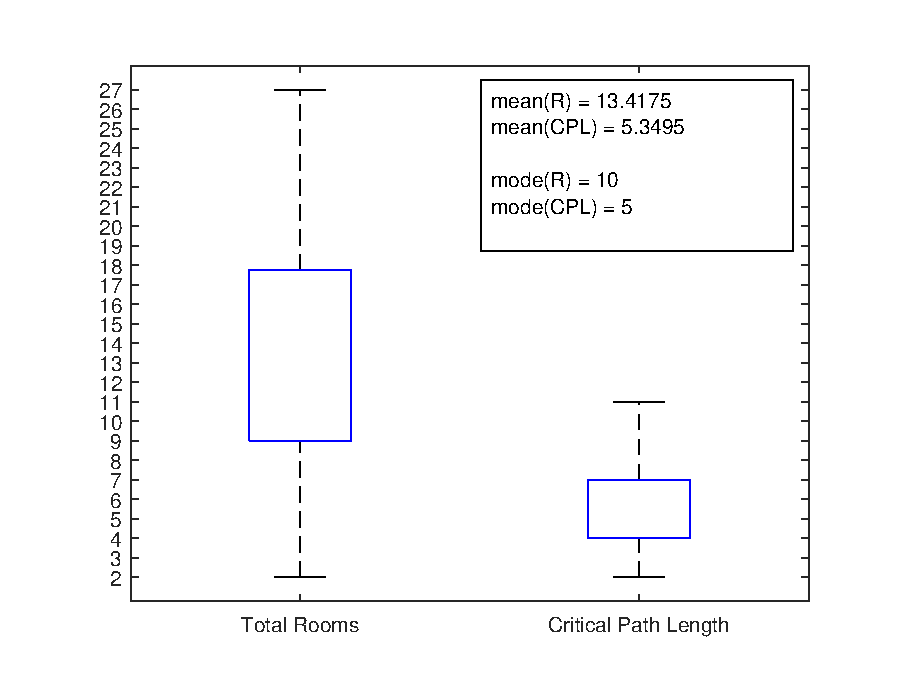
\includegraphics[width=\textwidth]{figures/data_plots/dungeon_bp.eps}
    \caption{Global (dungeon)}
  \end{subfigure}
  ~
  \begin{subfigure}[b]{0.45\textwidth}
    \centering
    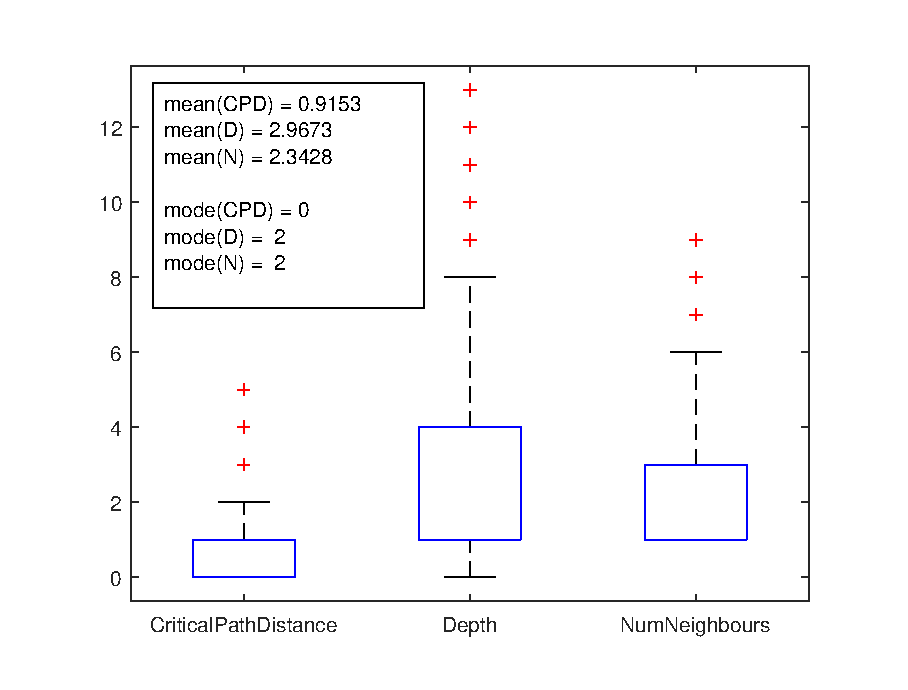
\includegraphics[width=\textwidth]{figures/data_plots/room_bp.eps}
    \caption{Local (Dungeon)}
  \end{subfigure}
  \caption{Parameter statistics}
  \label{fig:dataStats}
\end{figure}

\begin{algorithm}
  \SetAlgoLined
  \DontPrintSemicolon
  \SetKwFunction{Observe}{Observe}\SetKwFunction{Sample}{Sample}\SetKwFunction{ClearObservations}{ClearObservations}
  \SetKwInOut{Input}{input}\SetKwInOut{Output}{output}
  \Input{BNetModel, int \(observed\_R\)}
  \Output{int estimates for the dungeon and each room parameter \((R, L, \{S_r, D_r, N_r\})\)}
  \BlankLine
  \(isDungeonValid \leftarrow false\)\;
  \While{\(\neg isDungeonValid\)}{
    \(R \leftarrow \) BNetModel.\Observe{\(observed\_R\)}\;
    \(L \leftarrow \) BNetModel.\Sample{}\;
    \(isDungeonValid \leftarrow ValidateDungeon(R,L)\)\;
    \If{\(isDungeonValid\)}{
      \For{\(r \in R\) \KwDo}{
      \(temp\_R \leftarrow R\)\;
      \(temp\_L \leftarrow L\)\;
      \(isRoomValid \leftarrow false\)\;
      \While{\(\neg isRoomValid\)}{
        \((S_r, D_r, N_r) \leftarrow \) BNetModel.\Sample{}\;
        BNetModel.\ClearObservations{}\;
        \(R \leftarrow \) BNetModel.\Observe{\(temp\_R\)}\;
        \(L \leftarrow \) BNetModel.\Observe{\(temp\_L\)}\;
        \(isRoomValid \leftarrow ValidateRoom(S_r, D_r, N_r)\)\;
      }
    }
    }
   }
   \caption{Dungeon and Room sampling algorithm}
   \label{algo:sampling}
  \end{algorithm}

  \begin{algorithm}[H]
    \SetAlgoLined
    \DontPrintSemicolon
    \SetKwFunction{FMap}{Map}\SetKwFunction{FMapOne}{MapOne}\SetKwFunction{FPropagate}{Propagate}
    \SetKwFunction{FReduce}{Reduce}\SetKwFunction{FIsSingletonSet}{IsSingletonSet}\SetKwFunction{FUndo}{Undo}
    \SetKwFunction{FChooseRand}{ChooseRand}
    \SetKwProg{Fn}{Function}{:}{}
    \SetKwProg{try}{try}{}{}
    \SetKwProg{catch}{catch}{}{}
    \SetKwInOut{Input}{input}\SetKwInOut{Output}{output}
    \Input{set of rooms to be connected \(\mathcal{R}\), set of constraints for the dungeon and rooms \(\mathcal{C} = (R, L, \{S_r, D_r, N_r\})\)}
    \Output{A connected dungeon graph}
    
    \BlankLine
    \FMap{}\;

    \BlankLine
     \Fn{\FMap{}}{
      \For{\(r \in \mathcal{R}\)}{
        \(r_v \leftarrow\) all possible values for r\;
      }
      \FMapOne{}\;
      % \KwRet\;
     }

     \BlankLine
     %\tcc{Select a room \(r\) which still has more than one possible values in its set \(r_v\) and pick value for it}
     \Fn{\FMapOne{}}{
      \If{\(\forall r \mid\) \FIsSingletonSet{r_v}}{ %\If{} for normal ifs
        \KwRet\;
      }{
        \(r^\prime \leftarrow\) \FChooseRand{\(r \mid \)\FIsSingletonSet{\(r_v\)}}\;
        \For{\(v \in r^{\prime}_v\)}{
          \try{}
          {
            \FReduce{\(r^{\prime}_v, \{v\}\)}\;
            \FMapOne{}\;
          }
          \catch{\(Failure\)}{
            \FUndo{}\;
          }
        }
      }
      \;
     }

     \BlankLine
     \Fn{\FReduce{\(r_v, set\)}}{
      \If{\(set = \emptyset\)}{
        throw Failure\;
      }
      \If{\(r_v \ne set\)}{
        \(r_v \leftarrow set\)\;
        \For{\(c \in \mathcal{C}\)}{
          \FPropagate{\(c, r_v\)}\;
        }
      }
      % \KwRet\;
      \;
     }

     \BlankLine
     \Fn{\FPropagate{\(c, r^{\prime}_v\)}}{
      \For{\(r_v \in c_r\)}{
        \If{\(r_v \ne r^{\prime}_v\)}{
          \FReduce{\(r_v\),\FRemainingPossibilities{\(c, r_v\)}}\;
        }
      }
      % \KwRet\;
      \;
     }

     \caption{Constraint Propagation algorithm}
     \label{algo:CSP}
    \end{algorithm}

\chapter{Appendix}
\label{cha:aB}
\begin{figure}[htb]
  \centering
    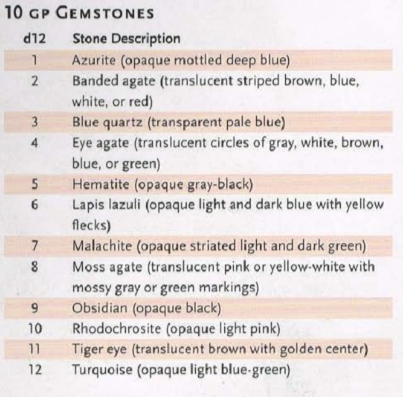
\includegraphics[width=0.5\textwidth]{figures/gemstone_table.png}
    \caption{Loot table for gemstones taken from Dungeon Master Guide 5e}
    \label{fig:loot_table}
\end{figure}

\begin{figure}[htb]
  \centering
  \begin{subfigure}[b]{0.45\textwidth}
    \centering
    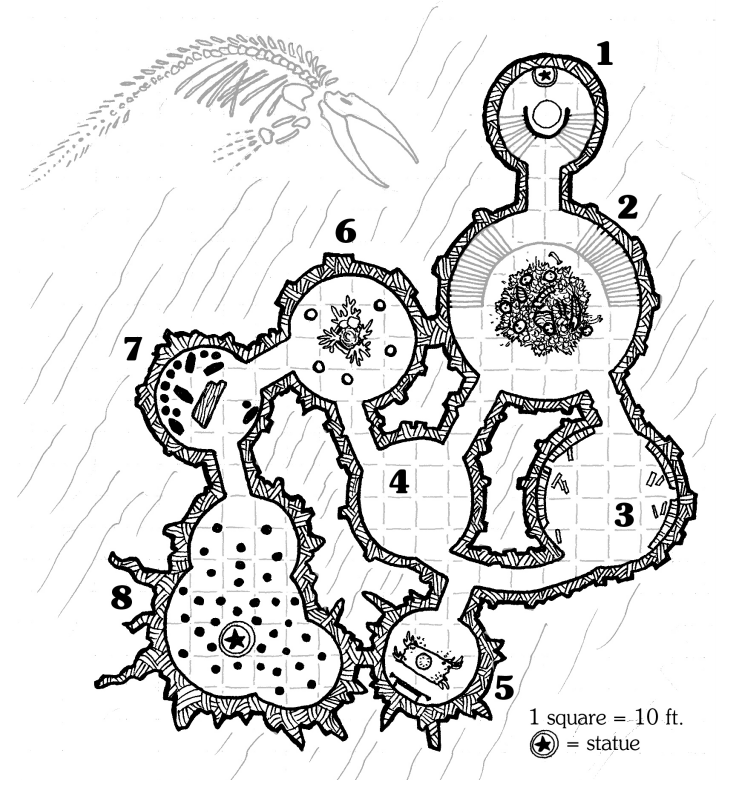
\includegraphics[width=\textwidth]{figures/step1.png}
    \caption{select a dungeon map}
  \end{subfigure}
  ~
  \begin{subfigure}[b]{0.45\textwidth}
    \centering
    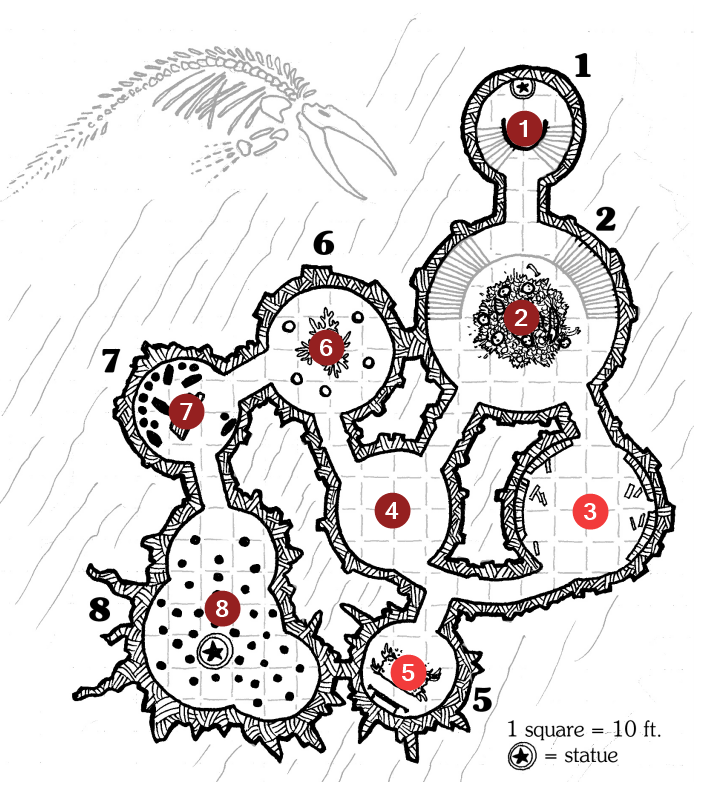
\includegraphics[width=\textwidth]{figures/step2.png}
    \caption{annotate (or reannotate) rooms for convenience}
  \end{subfigure}
  ~
  \begin{subfigure}[b]{0.45\textwidth}
    \centering
    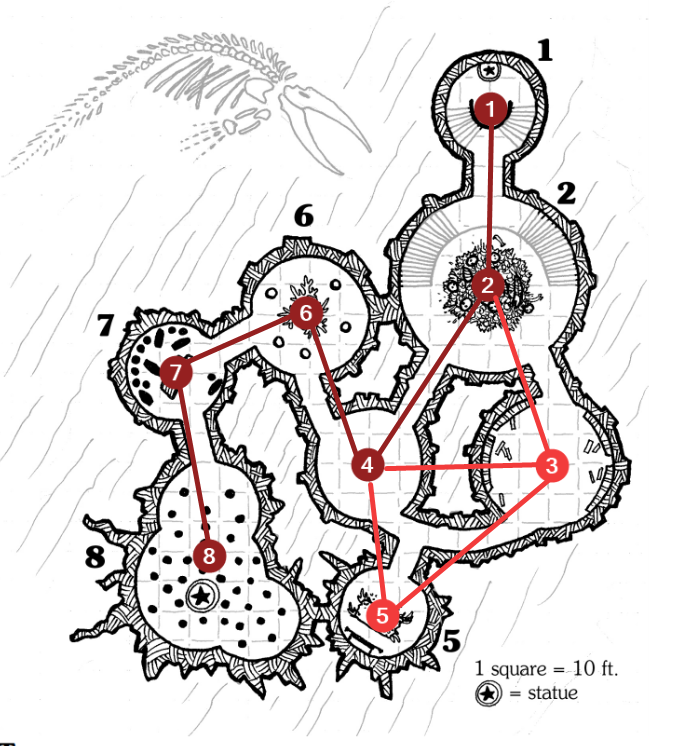
\includegraphics[width=\textwidth]{figures/step3.png}
    \caption{connect rooms}
  \end{subfigure}
  \caption{Steps for transcribing Sepulchre of the Abyss 2015 (dark red is CP)}
  \label{fig:SOTA}
\end{figure}

\begin{figure}[htb]
  \centering
  \begin{subfigure}[b]{0.45\textwidth}
    \centering
    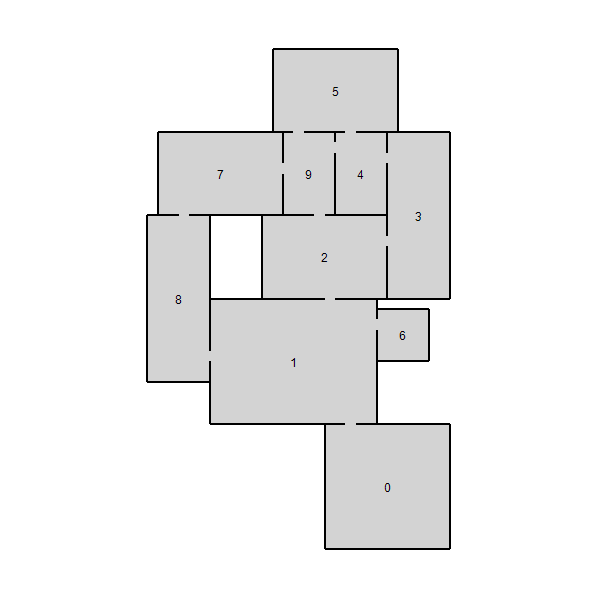
\includegraphics[width=\textwidth]{figures/generated/BPDG_10_5.jpg}
    \caption{10 room Bayesian PDG}
  \end{subfigure}
  ~
  \begin{subfigure}[b]{0.45\textwidth}
    \centering
    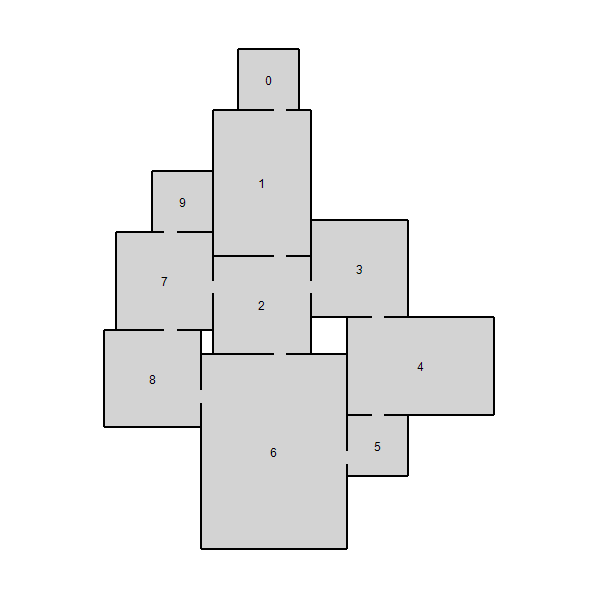
\includegraphics[width=\textwidth]{figures/generated/TheVerminHollow.yaml_7.jpg}
    \caption{The Vermin Hollow OPDC 2011}
  \end{subfigure}
  ~
  \begin{subfigure}[b]{0.45\textwidth}
    \centering
    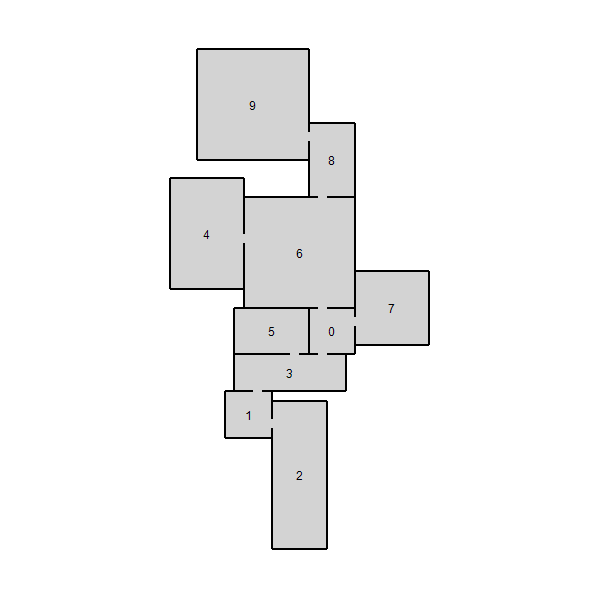
\includegraphics[width=\textwidth]{figures/generated/RAND_10_6.jpg}
    \caption{10 room Random PDG}
  \end{subfigure}
  \caption{Generated dungeons}
  \label{fig:gen_dungeons}
\end{figure}

\section{Preference Study Results}
\label{app:preference_study_results}

\begin{figure}[htb]
  \centering
  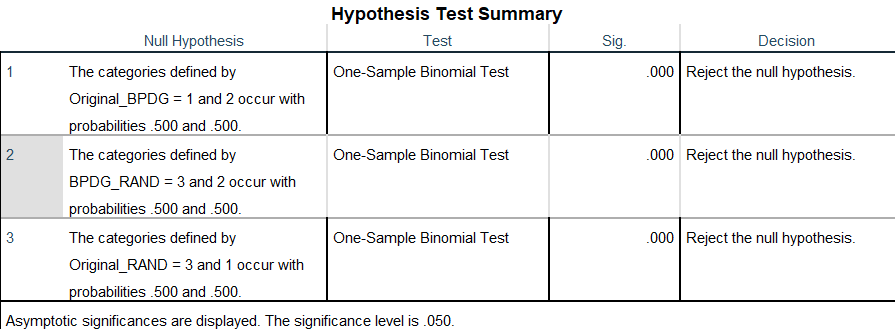
\includegraphics[width=\textwidth]{ExternalValidation/hypothesis_test_summary.png}
  \caption{significance test summary}
  \label{fig:binomial_test_summary}
\end{figure}

  \begin{figure}[htb]
    \centering
    \begin{subfigure}[b]{0.45\textwidth}
      \centering
      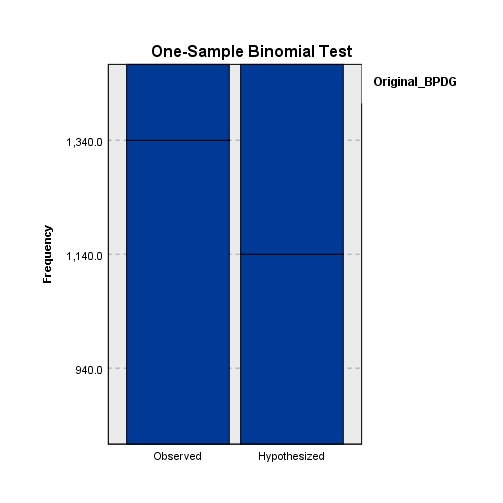
\includegraphics[width=\textwidth]{ExternalValidation/original_bpdg.png}
    \end{subfigure}
    ~
    \begin{subfigure}[b]{0.45\textwidth}
      \centering
      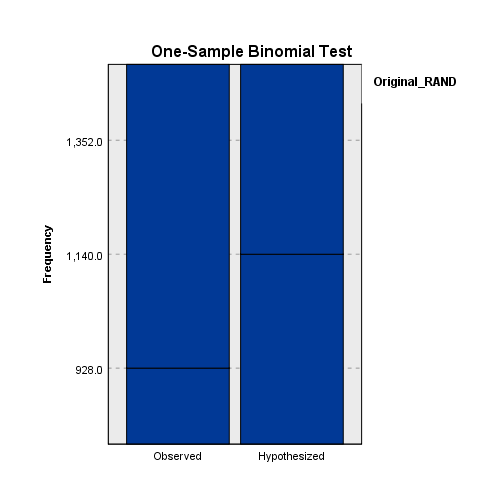
\includegraphics[width=\textwidth]{ExternalValidation/original_rand.png}
    \end{subfigure}
    ~
    \begin{subfigure}[b]{0.45\textwidth}
      \centering
      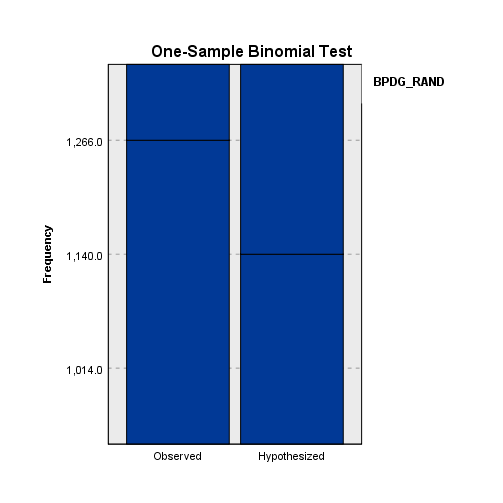
\includegraphics[width=\textwidth]{ExternalValidation/bpdg_rand.png}
    \end{subfigure}
    \caption{Hypothesised vs Actual distribution}
    \label{fig:hypothesised_vs_actual}
  \end{figure}

  \begin{figure}[htb]
    \centering
    \begin{subfigure}[b]{0.45\textwidth}
      \centering
      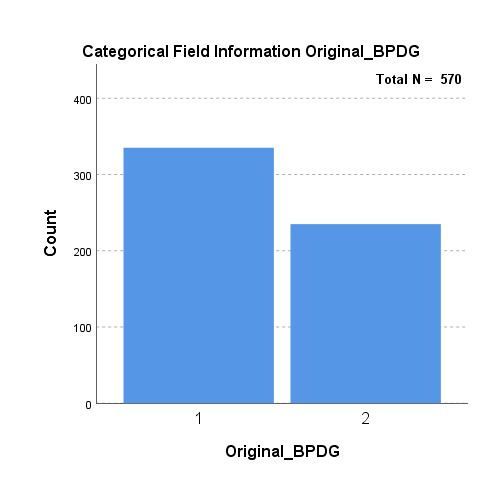
\includegraphics[width=\textwidth]{ExternalValidation/cat_info_original_bpdg.png}
    \end{subfigure}
    ~
    \begin{subfigure}[b]{0.45\textwidth}
      \centering
      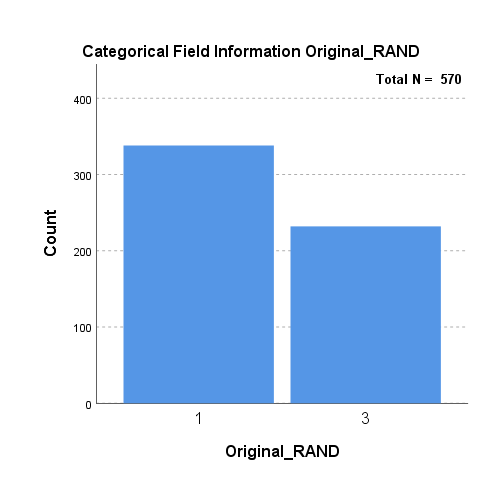
\includegraphics[width=\textwidth]{ExternalValidation/cat_info_original_rand.png}
    \end{subfigure}
    ~
    \begin{subfigure}[b]{0.45\textwidth}
      \centering
      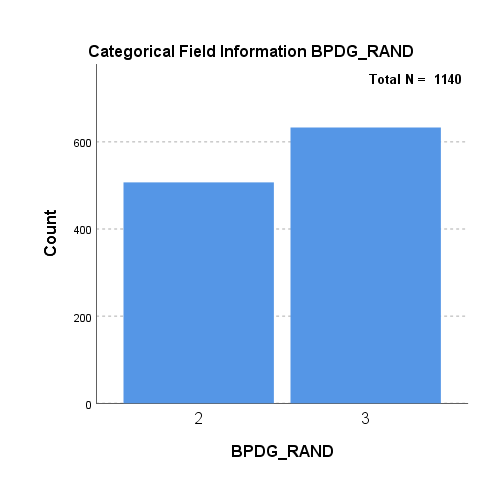
\includegraphics[width=\textwidth]{ExternalValidation/cat_info_bpdg_rand.png}
    \end{subfigure}
    \caption{Choice distributions}
    \label{fig:choice_distr}
  \end{figure}


\printbibliography

\end{document}